
\documentclass[12pt]{revtex4-1}
\usepackage{amssymb} % see geometry.pdf on how to lay out the page. There's lots.
%\geometry{a4paper} % or letter or a5paper or ... etc
% \geometry{landscape} % rotated page geometry
\usepackage{eqnarray,amsmath}
\usepackage{graphicx}



% See the ``Article customise'' template for come common customisations

\title{Kinoform Calculations}

%%% BEGIN DOCUMENT
\begin{document}

\maketitle

\section{Ideal Phase Pattern}
We are trying to replicate the phase pattern
\begin{equation}
\Psi = k_{\perp}r+m\phi
\end{equation}
with a kinoform in order to produce a high-order Bessel laser beam. First, we need to show that this phase pattern does in fact deliver a Bessel beam. 

\begin{figure}[tbh]
\centering
\begin{minipage}[t]{.45\textwidth}
\centering
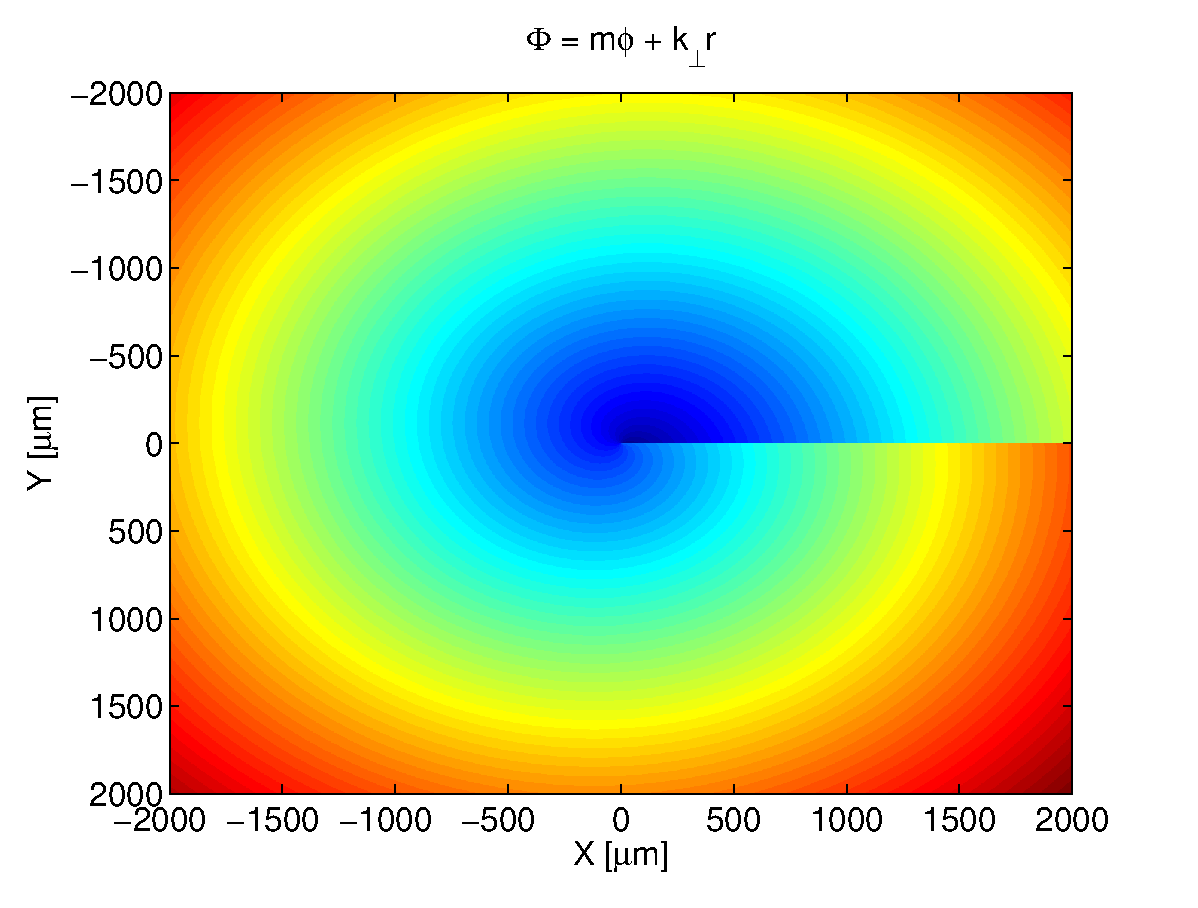
\includegraphics[width=.8\textwidth,height=4cm]{phase_func.eps}
\caption{Assumed input phase function.}
\end{minipage}\hfill
\begin{minipage}[t]{.45\textwidth}
\centering
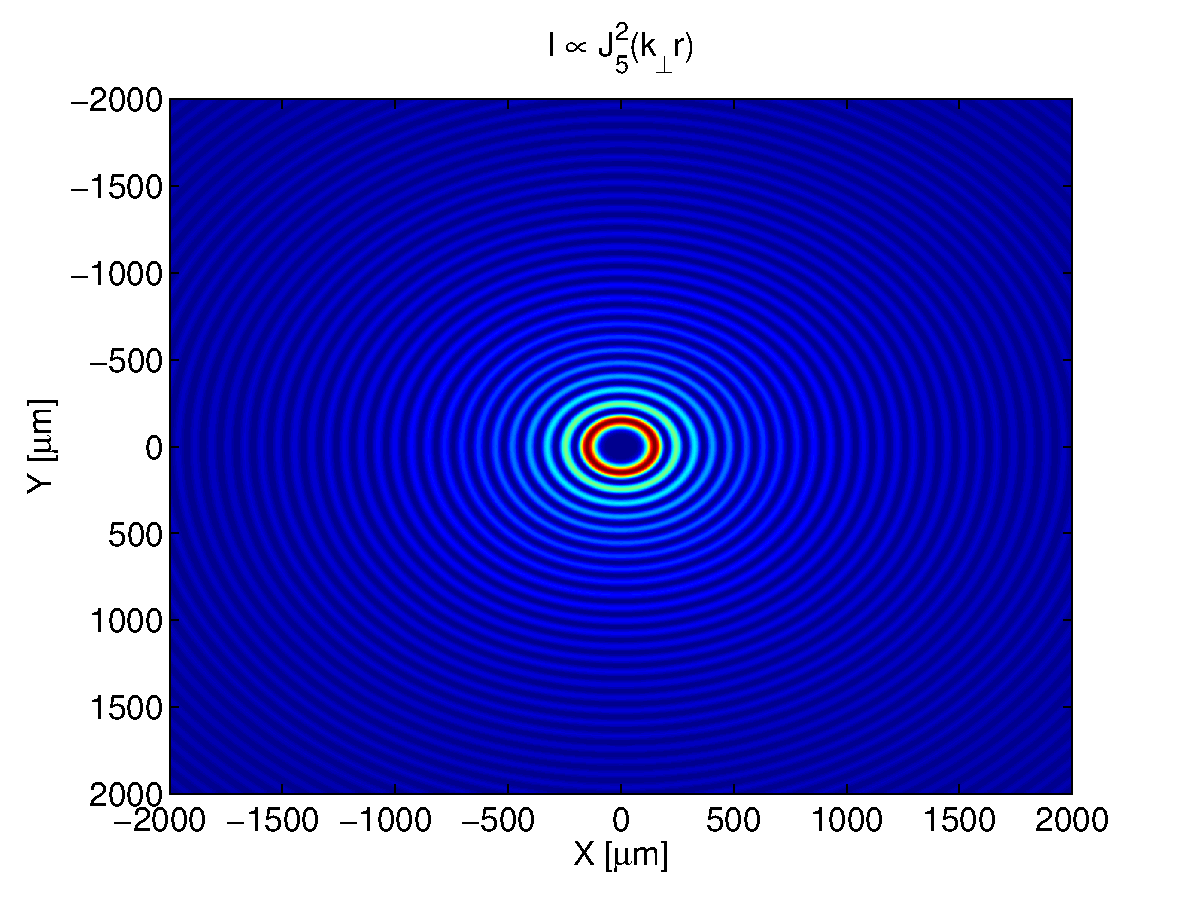
\includegraphics[width=.8\textwidth,height=4cm]{ideal_intensity.eps}
\caption{Ideal intensity function.}
\end{minipage}
\end{figure}

We assume that the incoming laser pulse is flat and uniform with radius $R$ before it reaches the kinoform. We assume that the kinoform imposes the phase pattern $\Psi$ and does not attenuate the pulse. Next, we propagate the field
\begin{equation}
U_0(r,\phi,z=0) = E_0 e^{i(k_{\perp}r+m\phi)}
\end{equation}
to a point in the observation plane using the Huygens-Fresnel equation:
\begin{equation}
U(r,\phi,z) = \int_0^\infty r'dr' \int_0^{2\pi} d\phi' U_0(r',\phi')\frac{e^{ikr_{01}}}{r_{01}}\cos{\theta}
\end{equation}
where $r_{01}$ is the length of the vector from the integration point to the field point and $\cos\theta$ is the angle between $r_{01}$ and the incoming beam vector.

\begin{figure}[tbh]
    \includegraphics{Huygens-Fresnel_field.PNG}
    \caption{Geometry for field calculation}
\end{figure}

This integral cannot be evaluated analytically for our choice of $U_0$ and it takes a long time to calculate numerically because each field point in the image plane is calculated with an $N\times N$ integral and we may want to do the calculation for $N\times N$ points in the image plane, leading to an $N^4$ calculation.

We can simplify things slightly by using the Fresnel diffraction formula:
\begin{equation}
U(r,\phi,z) = \frac{e^{ikz}}{i\lambda z}\int_0^\infty r'dr' \int_0^{2\pi} d\phi'  U_0(r',\phi')e^{\frac{ik}{2z}(|\vec{r}-\vec{r}'|)^2}
\end{equation}
where $|\vec{r}-\vec{r}'|$ is the length of a 2D between source and image point. Expanding $r$ and $r'$ in terms of their local coordinates, we have:
\begin{align}
|\vec{r}-\vec{r}'| =& \vec{r}^2 + \vec{r}'^2 -2\vec{r}\cdot\vec{r}'\\
			=& r^2+r'^2-2rr'(\cos\phi'\cos\phi + \sin\phi'\sin\phi)\\
			=& r^2+r'^2-2rr'\cos(\phi'-\phi)
\end{align}
Now the integral Fresnel integral is:
\begin{equation}
U(r,\phi,z) = \frac{e^{ik(z+\frac{r^2}{2z})}}{i\lambda z}\int_0^\infty r'dr' \int_0^{2\pi} d\phi'  U_0(r',\phi')e^{\frac{ik}{2z}[r'^2-2rr'\cos(\phi'-\phi)]}
\end{equation}
Plugging in $U_0$ we get:
\begin{equation}
U(r,\phi,z) = \frac{e^{ik(z+\frac{r^2}{2z})}}{i\lambda z}\int_0^\infty r' e^{i(k_{\perp}r' + \frac{kr'^2}{2z})}dr' \int_0^{2\pi} d\phi'  e^{i[m\phi'-\frac{krr'}{z}\cos(\phi'-\phi)]}
\end{equation}
Using the following as the definition of the Bessel function of the first kind:
\begin{equation}
J_m(x) = \frac{1}{2\pi}\int_{0}^{2\pi} e^{i(m\phi-x\cos\phi)}d\phi
\end{equation}
we recognize the $\phi'$ portion of the Fresnel integral as exactly that (note that we can set $\phi = 0$ to calculate the radial field). We then have:
\begin{equation}
U(r,z) = \frac{e^{ik(z+\frac{r^2}{2z})}}{i\lambda z}\int_0^\infty 2\pi J_m\left(\frac{krr'}{z}\right) r' e^{i(k_{\perp}r' + \frac{kr'^2}{z})}dr' 
\end{equation}
This equation is the Hankel transform of the input field. The advantage of this equation, from a numerical standpoint, is that we have reduced a 2D problem to a 1D problem. However, there is no clean function that is the Hankel transfer of our input function, so this is a dead end analytically. If we still want an analytic answer, we have to cheat. . . which we will.

\section{Stationary Phase Analysis}
In order to get an analytical expression for the field strength, we need to make some vast simplifications. The basic idea of the stationary phase analysis is that only rays taking the geometric path defined $r_\gamma = z\tan\gamma \approx z\gamma$ contribute to the field at a given $z$ location. 

\begin{figure}[tbh]
    \includegraphics[width=0.5\textwidth]{kinoform_geom.png}
    \caption{Geometry for stationary phase analysis}
\end{figure}

We replace $r'$ everywhere in the integral, except in the exponent to simplify the expression:
\begin{equation}
U(r,z) = \frac{e^{ik(z+\frac{r^2}{2z})}}{i\lambda z}\int_0^\infty 2\pi J_m\left(\frac{krr_\gamma}{z}\right) r_\gamma e^{i(k_{\perp}r' + \frac{kr'^2}{z})}dr'
\end{equation}
Identifying $k_\perp = k\sin\gamma \approx k\gamma$ in the integral, we have
\begin{equation}
U(r,z) = \frac{2\pi r_\gamma e^{ik(z+\frac{r^2}{2z})}}{i\lambda z} J_m\left(\frac{krr_\gamma}{z}\right) \int_0^\infty e^{ik(r'\gamma + \frac{r'^2}{z})}dr'
\end{equation}
Next, we complete the square in the integral and pull out a constant phase factor:
\begin{equation}
U(r,z) = \frac{k r_\gamma e^{ik(z+\frac{r^2}{2z}-\frac{\gamma^2}{2})}}{i z} J_m\left(\frac{krr_\gamma}{z}\right) \int_0^\infty e^{\frac{ik}{2z}(r'+z\gamma)^2}dr'
\end{equation}
Finally, we extend the integral from $-\infty$ to $\infty$. ``But that's ridiculous!" you say. I know, I know.
\begin{equation}
U(r,z) = \frac{k r_\gamma e^{ik(z+\frac{r^2}{2z}-\frac{\gamma^2}{2})}}{i z} J_m\left(\frac{krr_\gamma}{z}\right)\left[\sqrt{\frac{\pi z}{k}}(1+i)\right]
\end{equation}
Finally, we are interested in $I(r,z) = |U(r,z)|^2$ which gives
\begin{equation}
I(r,z) = I_0 2 \pi \gamma^2 kz J_m^2(kr\gamma)
\end{equation}
after substituting in $r_\gamma = z\gamma$.

\section{Grating Effects}
If we want to determine the real intensity of light focused by the kinoform, we have to include diffraction effects. Diffraction effects come from the fact that there is a finite pixel size for creating these gratings. For the gratings we have, the pixel size is $3.33 \mu$m and the etch depth is 880 nm. The value of pixel $ij$ in the grating is determined by:
\begin{align*}
 p_{ij} &=
  \begin{cases}
   0        & \text{if } 0 \leq \mod(k_\perp r_{ij} + m \phi_{ij},2\pi) < \pi\\
   1        & \text{if } \pi \leq \mod(k_\perp r_{ij} + m \phi_{ij},2\pi) < 2\pi
  \end{cases}
\end{align*}
Where $r_{ij}$ is the radius of pixel $ij$ and $\phi_{ij}$ is the angle of pixel $ij$. For this diffraction grating, we'd like to know how much intensity ends up in the zeroth grating order.

\begin{figure}[tbh]
    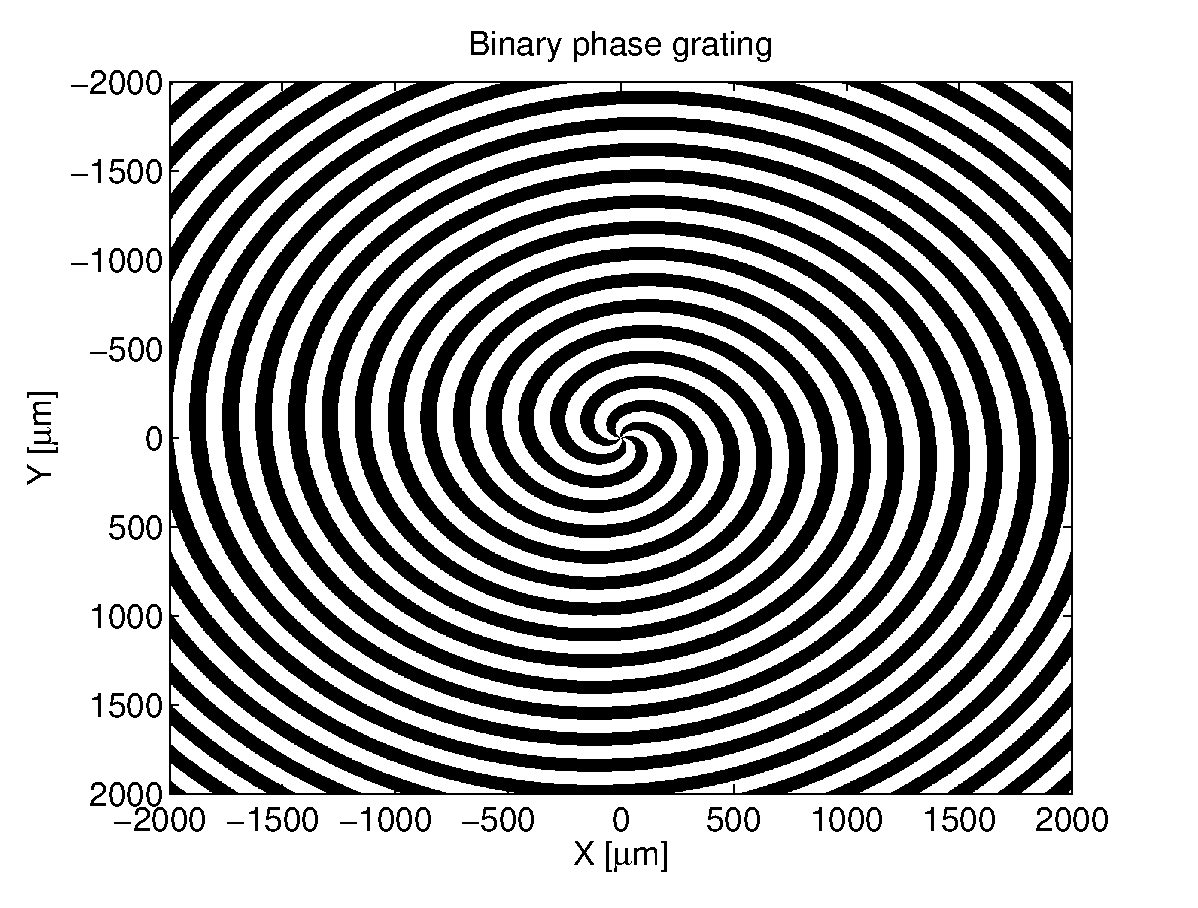
\includegraphics[width=0.5\textwidth]{mask.eps}
    \caption{Etching mask}
\end{figure}

\end{document}